\section{Cross section results}

This section presents the single differential particle level cross section results.
An extesive set of observables is shown in Figures ... through ....
The data points include statsitical uncertainties, as well as the full set of systematic uncertainties
discussed in chapter....

The data are compared to the MC event generators. 
Powheg interfaced with the Pythia parton shower.is shown in the DR and DS schemes,
alongside Powheg employing the alternative Herwig parton shower.
For a quantative comparison, the $\chi^2$ values are provided in Table ... for every observable and theory prediction.



\vspace{.5cm}
\noindent
\textbf{WWbb kinematics}
\vspace{.5cm}

\noindent
Selected observables determining the kinematics of the $WWbb$ process are collected in Figure \dots
The uncertainties are dominated by \dots
Data MC agreement within uncertainties
Trend to overestimate the data at large momenta in all three models.

\begin{figure}[ht!]
	\centering
	\begin{subfigure}[b]{0.42\linewidth}
		\includegraphics[width=1.\linewidth, page=5]{figures/WbWb/WhadParticle/paper_observables/final_unfolded_TUnfoldStandalone_OptionA_data_nonClosureAlternative_SR_Whad_Final_l_Whad_particle.pdf}
		\caption{\mbox{}}
		\label{fig:whadpart:xsec:pt_lep}
	\end{subfigure}
	\begin{subfigure}[b]{0.42\linewidth}
		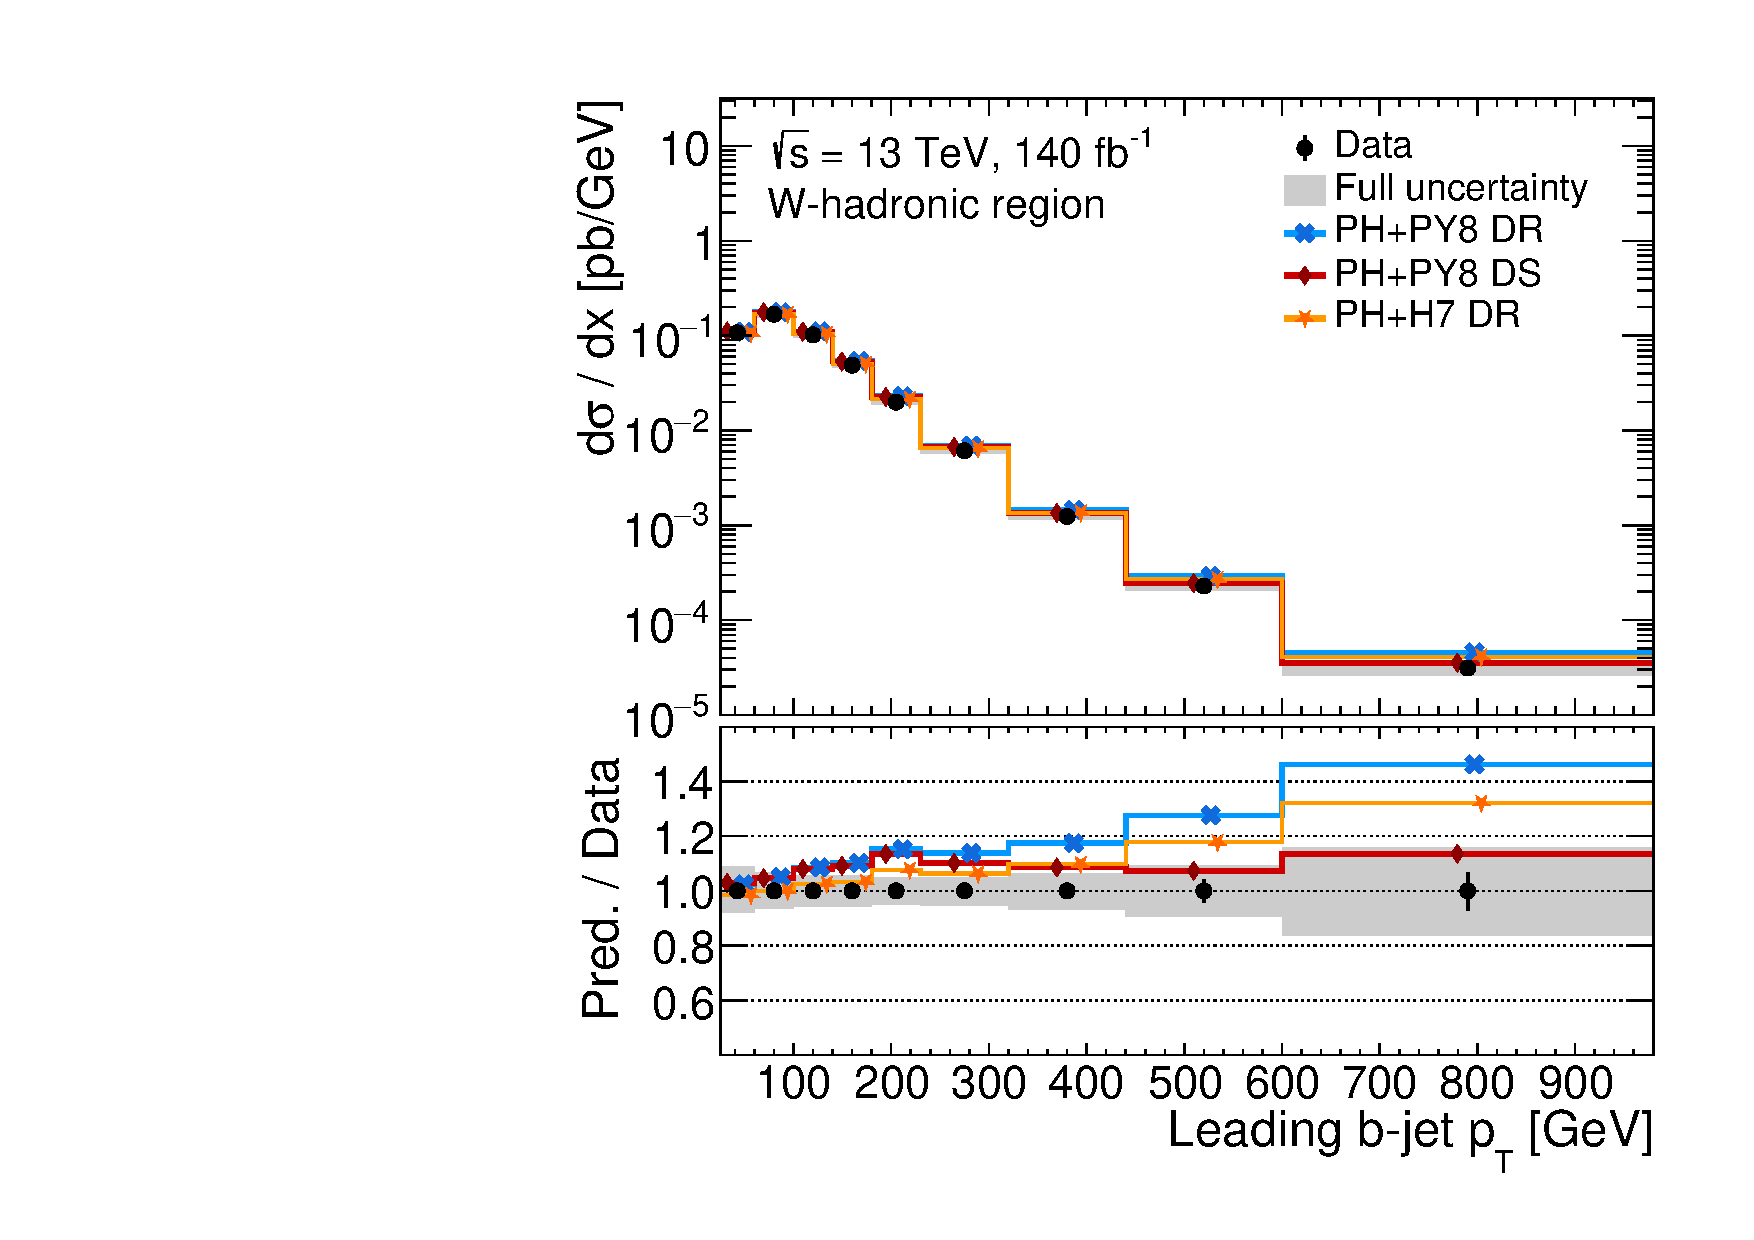
\includegraphics[width=1.\linewidth, page=1]{figures/WbWb/WhadParticle/paper_observables/final_unfolded_TUnfoldStandalone_OptionA_data_nonClosureAlternative_SR_Whad_Final_l_Whad_particle.pdf}
		\caption{\mbox{}}
		\label{fig:whadpart:xsec:pt_bjet1}
	\end{subfigure}
    \\
	\begin{subfigure}[b]{0.42\linewidth}
		\includegraphics[width=1.\linewidth, page=5]{figures/WbWb/WhadParticle/more_observables/final_unfolded_TUnfoldStandalone_OptionA_data_nonClosureAlternative_SR_Whad_Final_l_Whad_particle.pdf}
		\caption{\mbox{}}
		\label{fig:whadpart:xsec:pt_w}
	\end{subfigure}
	\begin{subfigure}[b]{0.42\linewidth}
		\includegraphics[width=1.\linewidth, page=6]{figures/WbWb/WhadParticle/paper_observables/final_unfolded_TUnfoldStandalone_OptionA_data_nonClosureAlternative_SR_Whad_Final_l_Whad_particle.pdf}
		\caption{\mbox{}}
		\label{fig:whadpart:xsec:m_bl}
	\end{subfigure}
	\caption{Cross sections.}
	\label{fig:whadpart:xsec:selected}
\end{figure}

\vspace{.5cm}
\noindent
\textbf{Towards the top mass}
\vspace{.5cm}

\noindent
Show selected quantities which are sensitive to the top quark mass or can be used to constrain systematic uncertainties

\begin{figure}[ht!]
	\centering
	\begin{subfigure}[b]{0.3\linewidth}
		\includegraphics[width=1.\linewidth, page=2]{figures/WbWb/WhadParticle/paper_observables/final_unfolded_TUnfoldStandalone_OptionA_data_nonClosureAlternative_SR_Whad_Final_l_Whad_particle.pdf}
		\caption{\mbox{}}
		\label{fig:whadpart:xsec:pt_bjet2}
	\end{subfigure}
	\begin{subfigure}[b]{0.3\linewidth}
		\includegraphics[width=1.\linewidth, page=3]{figures/WbWb/WhadParticle/paper_observables/final_unfolded_TUnfoldStandalone_OptionA_data_nonClosureAlternative_SR_Whad_Final_l_Whad_particle.pdf}
		\caption{\mbox{}}
		\label{fig:whadpart:xsec:pt_owj1}
	\end{subfigure}
	\begin{subfigure}[b]{0.3\linewidth}
		\includegraphics[width=1.\linewidth, page=4]{figures/WbWb/WhadParticle/paper_observables/final_unfolded_TUnfoldStandalone_OptionA_data_nonClosureAlternative_SR_Whad_Final_l_Whad_particle.pdf}
		\caption{\mbox{}}
		\label{fig:whadpart:xsec:pt_owj2}
	\end{subfigure}
    \\
	\begin{subfigure}[b]{0.3\linewidth}
		\includegraphics[width=1.\linewidth, page=2]{figures/WbWb/WhadParticle/more_observables/final_unfolded_TUnfoldStandalone_OptionA_data_nonClosureAlternative_SR_Whad_Final_l_Whad_particle.pdf}
		\caption{\mbox{}}
		\label{fig:whadpart:xsec:pt_met}
	\end{subfigure}
    	\begin{subfigure}[b]{0.3\linewidth}
		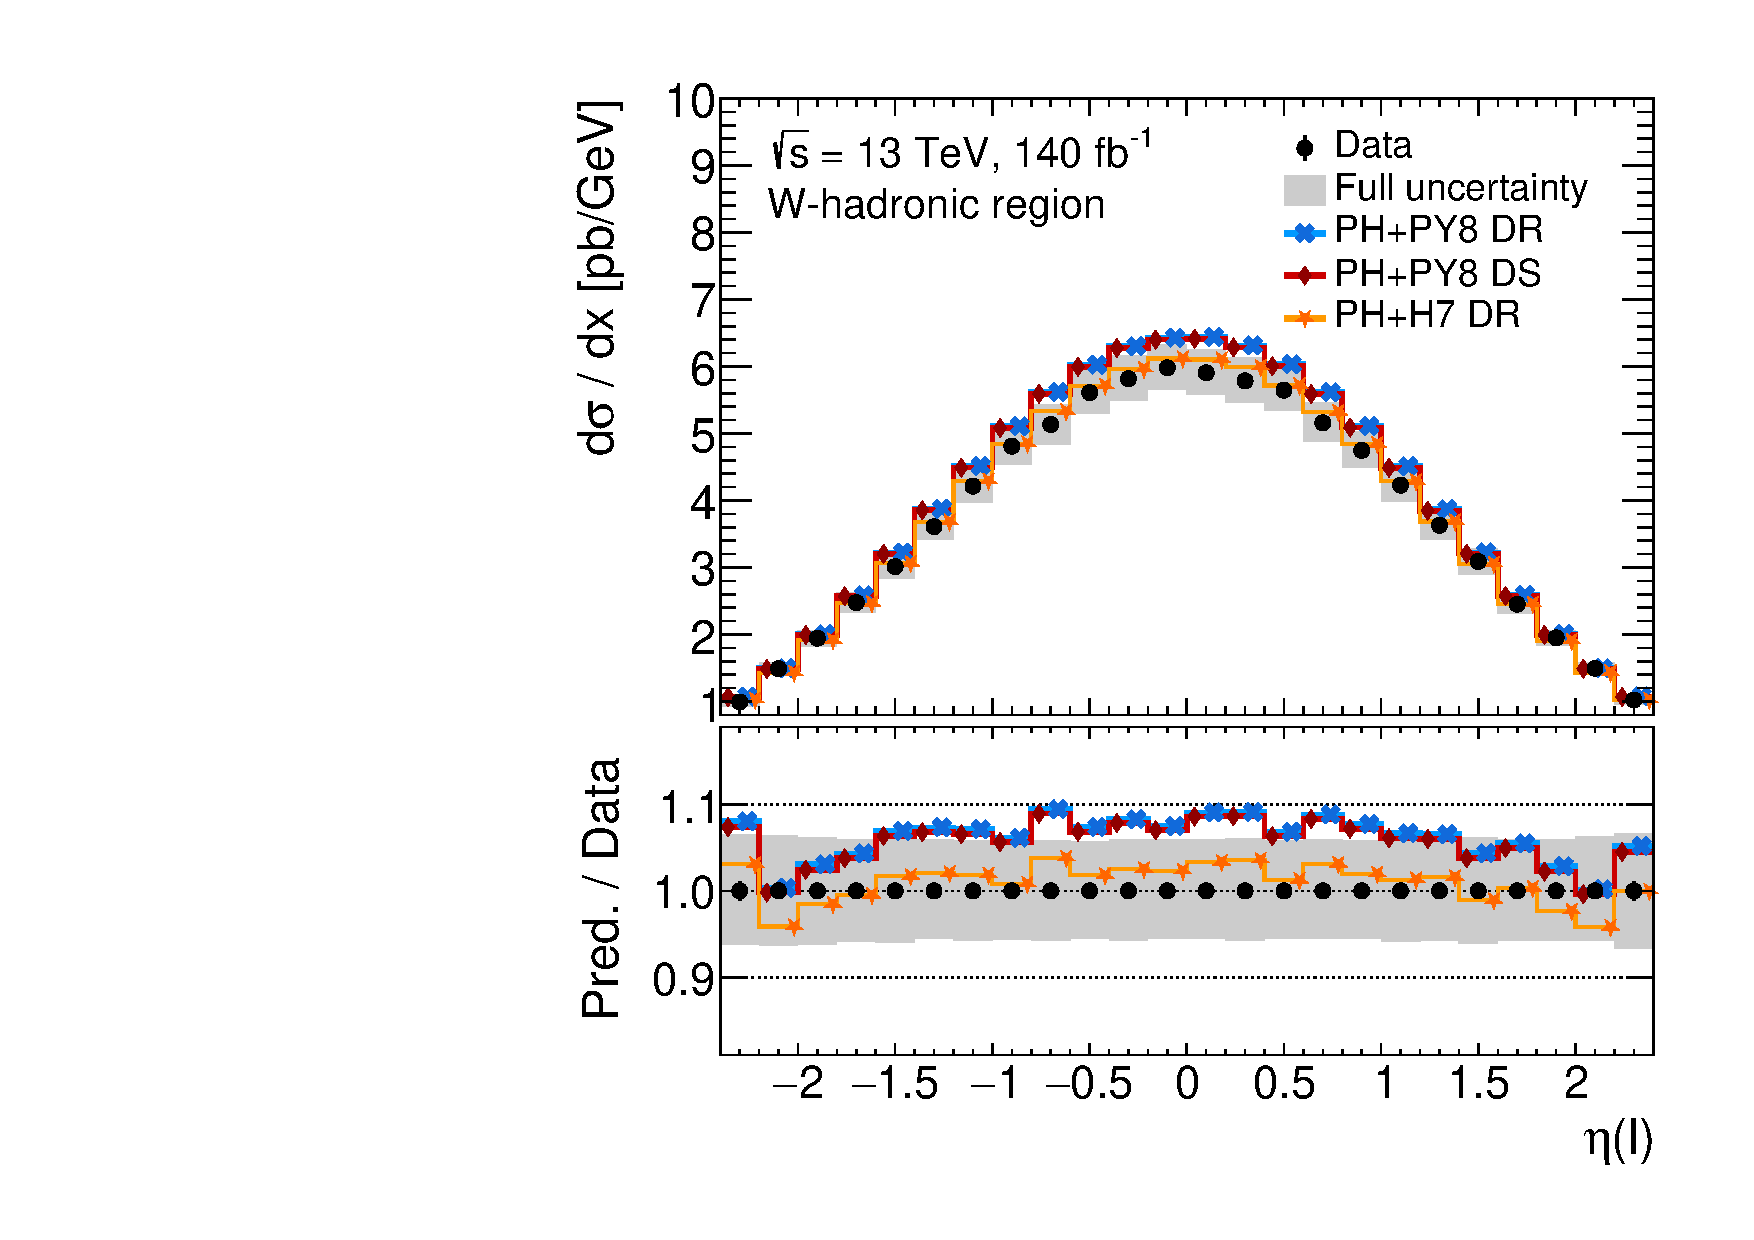
\includegraphics[width=1.\linewidth, page=1]{figures/WbWb/WhadParticle/more_observables/final_unfolded_TUnfoldStandalone_OptionA_data_nonClosureAlternative_SR_Whad_Final_l_Whad_particle.pdf}
		\caption{\mbox{}}
		\label{fig:whadpart:xsec:etal}
	\end{subfigure}
	\begin{subfigure}[b]{0.3\linewidth}
		\includegraphics[width=1.\linewidth, page=6]{figures/WbWb/WhadParticle/more_observables/final_unfolded_TUnfoldStandalone_OptionA_data_nonClosureAlternative_SR_Whad_Final_l_Whad_particle.pdf}
		\caption{\mbox{}}
		\label{fig:whadpart:xsec:yw}
	\end{subfigure}
    \\
        \begin{subfigure}[b]{0.3\linewidth}
		\includegraphics[width=1.\linewidth, page=12]{figures/WbWb/WhadParticle/more_observables/final_unfolded_TUnfoldStandalone_OptionA_data_nonClosureAlternative_SR_Whad_Final_l_Whad_particle.pdf}
		\caption{\mbox{}}
		\label{fig:whadpart:xsec:rbq}
	\end{subfigure}
	\begin{subfigure}[b]{0.3\linewidth}
		\includegraphics[width=1.\linewidth, page=13]{figures/WbWb/WhadParticle/more_observables/final_unfolded_TUnfoldStandalone_OptionA_data_nonClosureAlternative_SR_Whad_Final_l_Whad_particle.pdf}
		\caption{\mbox{}}
		\label{fig:whadpart:xsec:rbj}
	\end{subfigure}
	\caption{Basic plots \pt and other stuff.}
	\label{fig:whadpart:xsec:pt}
\end{figure}


\begin{figure}[ht!]
	\centering
	\begin{subfigure}[b]{0.3\linewidth}
		\includegraphics[width=1.\linewidth, page=9]{figures/WbWb/WhadParticle/paper_observables/final_unfolded_TUnfoldStandalone_OptionA_data_nonClosureAlternative_SR_Whad_Final_l_Whad_particle.pdf}
		\caption{\mbox{}}
		\label{fig:whadpart:xsec:pt_bw}
	\end{subfigure}
   	\begin{subfigure}[b]{0.3\linewidth}
		\includegraphics[width=1.\linewidth, page=8]{figures/WbWb/WhadParticle/paper_observables/final_unfolded_TUnfoldStandalone_OptionA_data_nonClosureAlternative_SR_Whad_Final_l_Whad_particle.pdf}
		\caption{\mbox{}}
		\label{fig:whadpart:xsec:mbw}
	\end{subfigure}
	\begin{subfigure}[b]{0.3\linewidth}
		\includegraphics[width=1.\linewidth, page=13]{figures/WbWb/WhadParticle/paper_observables/final_unfolded_TUnfoldStandalone_OptionA_data_nonClosureAlternative_SR_Whad_Final_l_Whad_particle.pdf}
		\caption{\mbox{}}
		\label{fig:whadpart:xsec:drbw}
	\end{subfigure}
    \\
    \begin{subfigure}[b]{0.3\linewidth}
		\includegraphics[width=1.\linewidth, page=7]{figures/WbWb/WhadParticle/paper_observables/final_unfolded_TUnfoldStandalone_OptionA_data_nonClosureAlternative_SR_Whad_Final_l_Whad_particle.pdf}
		\caption{\mbox{}}
		\label{fig:whadpart:xsec:pt_bl}
	\end{subfigure}
    	\begin{subfigure}[b]{0.3\linewidth}
		\includegraphics[width=1.\linewidth, page=12]{figures/WbWb/WhadParticle/paper_observables/final_unfolded_TUnfoldStandalone_OptionA_data_nonClosureAlternative_SR_Whad_Final_l_Whad_particle.pdf}
		\caption{\mbox{}}
		\label{fig:whadpart:xsec:drbl}
	\end{subfigure}
	\begin{subfigure}[b]{0.3\linewidth}
		\includegraphics[width=1.\linewidth, page=9]{figures/WbWb/WhadParticle/more_observables/final_unfolded_TUnfoldStandalone_OptionA_data_nonClosureAlternative_SR_Whad_Final_l_Whad_particle.pdf}
		\caption{\mbox{}}
		\label{fig:whadpart:xsec:pt_blnu}
	\end{subfigure}
    \\
    \begin{subfigure}[b]{0.3\linewidth}
		\includegraphics[width=1.\linewidth, page=10]{figures/WbWb/WhadParticle/more_observables/final_unfolded_TUnfoldStandalone_OptionA_data_nonClosureAlternative_SR_Whad_Final_l_Whad_particle.pdf}
		\caption{\mbox{}}
		\label{fig:whadpart:xsec:pt_wbbl}
	\end{subfigure}
	\begin{subfigure}[b]{0.3\linewidth}
		\includegraphics[width=1.\linewidth, page=10]{figures/WbWb/WhadParticle/paper_observables/final_unfolded_TUnfoldStandalone_OptionA_data_nonClosureAlternative_SR_Whad_Final_l_Whad_particle.pdf}
		\caption{\mbox{}}
		\label{fig:whadpart:xsec:mwbbl}
	\end{subfigure}
    \begin{subfigure}[b]{0.3\linewidth}
		\includegraphics[width=1.\linewidth, page=11]{figures/WbWb/WhadParticle/more_observables/final_unfolded_TUnfoldStandalone_OptionA_data_nonClosureAlternative_SR_Whad_Final_l_Whad_particle.pdf}
		\caption{\mbox{}}
		\label{fig:whadpart:xsec:pt_wbblnu}
	\end{subfigure}
    \\
	\begin{subfigure}[b]{0.3\linewidth}
		\includegraphics[width=1.\linewidth, page=11]{figures/WbWb/WhadParticle/paper_observables/final_unfolded_TUnfoldStandalone_OptionA_data_nonClosureAlternative_SR_Whad_Final_l_Whad_particle.pdf}
		\caption{\mbox{}}
		\label{fig:whadpart:xsec:minimax}
	\end{subfigure}
	\begin{subfigure}[b]{0.3\linewidth}
		\includegraphics[width=1.\linewidth, page=3]{figures/WbWb/WhadParticle/more_observables/final_unfolded_TUnfoldStandalone_OptionA_data_nonClosureAlternative_SR_Whad_Final_l_Whad_particle.pdf}
		\caption{\mbox{}}
		\label{fig:whadpart:xsec:mtl}
	\end{subfigure}
	\begin{subfigure}[b]{0.3\linewidth}
		\includegraphics[width=1.\linewidth, page=7]{figures/WbWb/WhadParticle/more_observables/final_unfolded_TUnfoldStandalone_OptionA_data_nonClosureAlternative_SR_Whad_Final_l_Whad_particle.pdf}
		\caption{\mbox{}}
		\label{fig:whadpart:xsec:mblmi}
	\end{subfigure}
%	\begin{subfigure}[b]{0.3\linewidth}
%		\includegraphics[width=1.\linewidth, page=8]{figures/WbWb/WhadParticle/more_observables/final_unfolded_TUnfoldStandalone_OptionA_data_nonClosureAlternative_SR_Whad_Final_l_Whad_particle.pdf}
%		\caption{\mbox{}}
%		\label{fig:whadpart:xsec:mtblmin}
%	\end{subfigure}
%	\caption{}
%	\label{fig:whadpart:xsec:mass}
	\caption{All other plots}
	\label{fig:whadpart:xsec:angles}
\end{figure}



\begin{table}[htbp]
    \centering
    \caption{Comparison of Generator Performance. Chi square calculation outlined in the text.}
    \resizebox{\textwidth}{!}{%
    \begin{tabular}{l|cccccccccccccccc}
        %\toprule
        & \multicolumn{6}{c}{\textbf{Generator}} \\
        %\cmidrule(lr){2-7}
        & \multicolumn{2}{c}{PH+ PYTHIA 8 (DR)} & \multicolumn{2}{c}{PH+ PYTHIA 8 (DS)} & \multicolumn{2}{c}{PH+ HERWIG 7.1 (DR)}\\
        %\cmidrule(lr){2-3} \cmidrule(lr){4-5} \cmidrule(lr){6-7}
        \textbf{Observable} & $\chi^2/\text{NDF}$ & p-value & $\chi^2/\text{NDF}$ & p-value & $\chi^2/\text{NDF}$ & p-value\\
        \midrule
        Lepton $p_T$ & 45.44 / 8 & $<0.001$ & 55.26 / 11 & $<0.001$ & 25.36 / 11 & 0.008 \\
        Leading $b$-jet $p_T$ & 30.59 / 12 & 0.002 & 41.35 / 12 & $<0.001$ & 24.28 / 12 & 0.019 \\
        Subleading $b$-jet $p_T$ & 32.76 / 9 & $<0.001$ & 36.88 / 9 & $<0.001$ & 27.33 / 9 & 0.001 \\
        Leading light-jet $p_T$ & 15.22 / 10 & 0.124 & 20.25 / 10 & 0.027 & 9.21 / 10 & 0.512 \\
        Hadronic-W $p_T$ & 17.87 / 11 & 0.085 & 22.70 / 11 & 0.019 & 12.03 / 11 & 0.362 \\
        Selected ($b + \ell$) mass & 21.04 / 20 & 0.395 & 33.20 / 20 & 0.032 & 41.95 / 20 & 0.003 \\
        Selected ($b + W_{\text{had.}}$) mass & 24.22 / 10 & 0.007 & 26.74 / 10 & 0.003 & 50.13 / 10 & $<0.001$ \\
        Selected ($W_{\text{had.}} + b_1 + b_2 + \ell$) mass & 4.08 / 9 & 0.906 & 4.01 / 9 & 0.911 & 5.08 / 9 & 0.827 \\
        Modified minimax mass & 18.96 / 10 & 0.041 & 25.95 / 10 & 0.004 & 45.30 / 10 & $<0.001$ \\
        Hadronic-W $y$ & 14.95 / 12 & 0.244 & 15.26 / 12 & 0.228 & 14.24 / 12 & 0.285\\
        $\Delta R(b, \ell)$ & 41.25 / 8 & $<0.001$ & 42.04 / 8 & $<0.001$ & 42.88 / 8 & $<0.001$\\
        $\Delta R(b, W_{\text{had.}})$ & 103.0 / 8 & $<0.001$ & 105.1 / 8 & $<0.001$ & 107.3 / 8 & $<0.001$\\
        %\bottomrule
    \end{tabular}%
    }
\end{table}

%To do: Polish plots
% - Remove ATLAS label (DONE)
% - Change label "W-hadronic region"
% - Change color scheme (DONE)
% - Decide which models to compare to the data (only DR and DS?)
% - Binning: mbw? / ptwbblnu (DONE)
% - y-axis range (also in ration plot) / log scale? (DONE)
% - x axis label ptwbblnu (DONE)
% 
% 